\section{Introduction}
\label{sec:introduction}

% state the learning objective 
The objective of this laboratory assignment is to study a circuit containing 7 resistors, a linear voltage source $V_a$, a linear current source $I_b$, a current induced voltage source $V_c$ and a voltage induced current source $I_b$. The circuit can be seen if Figure~\ref{fig:rc}.

%\lipsum[1-1]
\begin{figure}[h] \centering
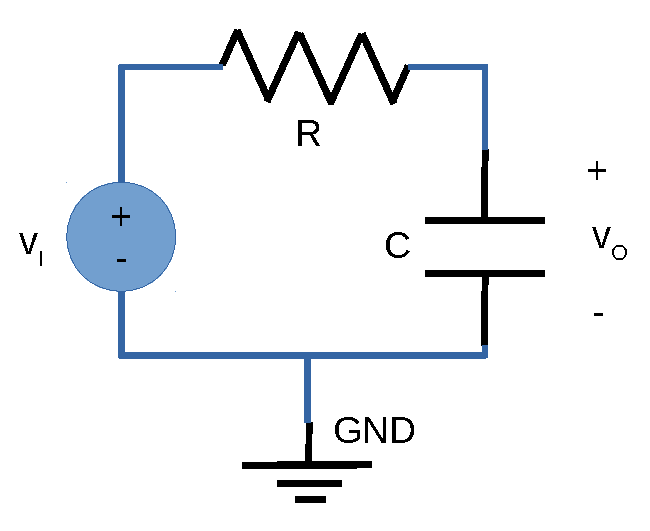
\includegraphics[width=0.6\linewidth]{rc.pdf}
\caption{The circuit under analysis.}
\label{fig:rc}
\end{figure}\label{fig:rc}

In Section \ref{sec:analysis}, a theoretical analysis of the circuit is
presented, accordingly to two distinct methods: mesh analysis and nodal analysis. In Section\ref{sec:simulation}, the circuit is analysed by
simulation, and the results are compared to the theoretical results obtained in
Section~\ref{sec:analysis}. The conclusions of this study are outlined in
Section~\ref{sec:conclusion}.





